\section{Auswertung}
\label{sec:auswertung}
In diesem Kapitel sollen die aufgenommenen Messwerte ausgewertet und in Beziehung gebracht werden.

\subsection{Der Einfachspalt}
\label{sec:einfachspalt}
Zunächst wurde eine Dunkelstrommesseung durchgeführt, dazu wurde im abgedunkelten Raum bei ausgeschaltetem
Laser der Detektorstrom $I_D$ gemessen. Er belauft sich auf:
\begin{center}
    $I_D=10\times 10^{-9}\si[]{A}$
\end{center}
Zudem wurde noch der Abstand zwischen beugendem Element und Detekor zu $z=1.05\si[]{m}$ bestimmt.
Der Beugungswinkel $\phi$ ergibt sich über die Beziehung:
\begin{center}
    $\phi=arctan(\frac{x_1}{z})$
\end{center}
wobei $x_1$ den Abstand vom Intensitätsmaximum beschreibt.
An die Messwerte wurde mittels der Python scipy Bibliothek eine Kurve nach \autoref{eq:einfachspalt} 
angepasst, das Ergebnis ist in \autoref{fig:es} zu sehen. Es wurden dabei folgende Parameter verwendet:
\begin{center}
    $A_0=325.98\pm 27.204$\\
    $b=0.855\pm 0.085\si[]{mm}$
\end{center}
\begin{figure}
    \centering
    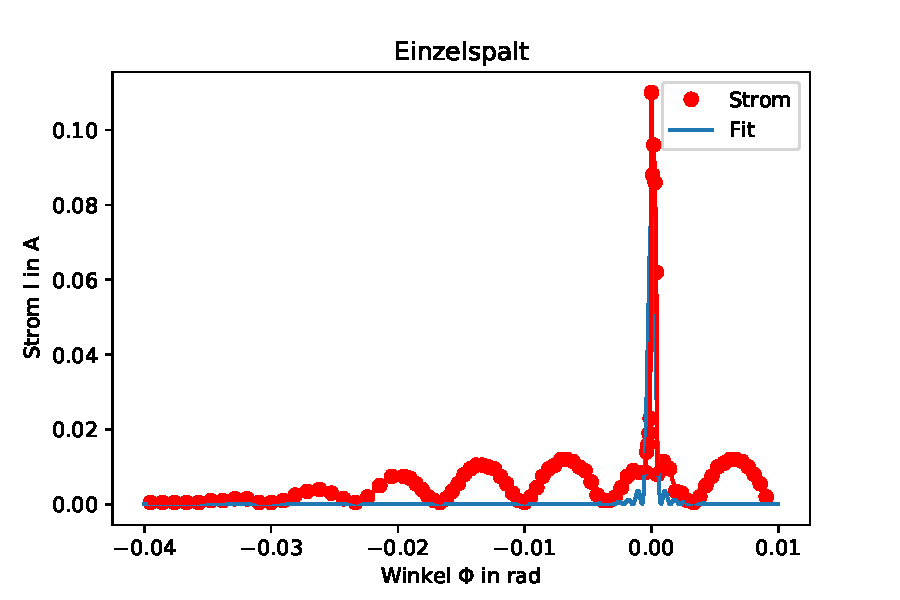
\includegraphics{Einzelspalt.pdf}
    \caption{Beugungsmuster am Einzelspalt}
    \label{fig:es}
  \end{figure}

\subsection{Doppelspalt}
\label{sec:doppelspalt}
Um den Doppelspalt zu untersuchen wurde die selbe Apperatur benutzt, daher bleiben die Werte für $z$
und $I_D$ gleich. Ebenfalls wurde der Beugungswinkel auch in diesem Kapitel wie \autoref{sec:einfachspalt}
berechnet. An die erhaltenen Messdaten wurde eine Kurve nach \autoref{eq:doppelspalt} angepasst. Die 
erhaltenen Werte wurden dann in die Funktion \autoref{eq:einfachspalt} eingesetzt um die Einhüllende zu erhalten.
Das Ergebnis ist in \autoref{fig:ds} zu sehen. Es fällt auf das die Kurve des Einzelspaltes die des Doppelspaltes sehr gut 
umreißt. Das Bestätigt die Annahme das der Doppelspalt als überlagerung zweier Einzelspalt-Beugungsbilder beschrieben werden kann.

\end{description}
\begin{figure}
    \centering
    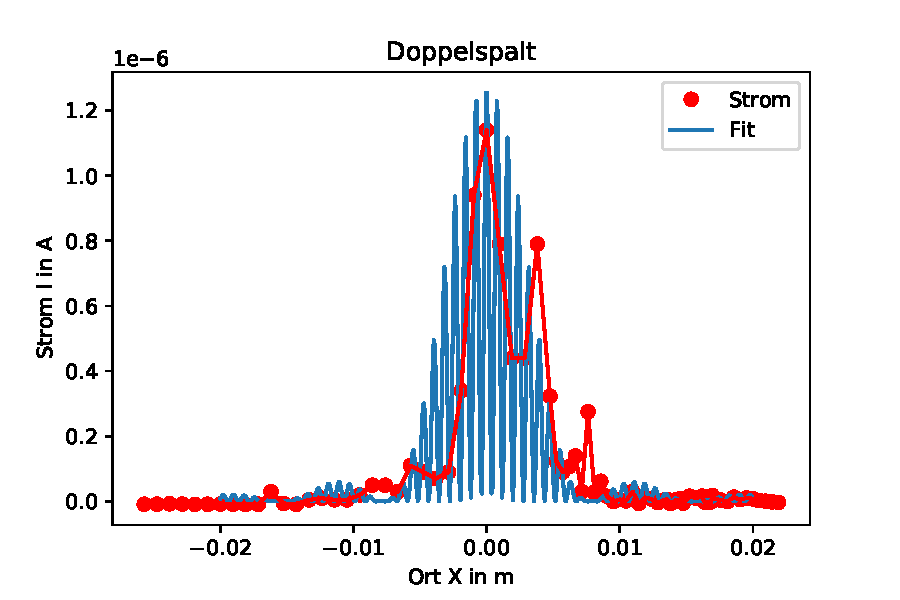
\includegraphics{doppelspalt.pdf}
    \caption{Beugungsmuster mit Einhüllender am Doppelspalt}
    \label{fig:ds}
  \end{figure}

Durch die Ausgleichsrechnung ergaben sich folgende Werte:
\begin{center}
    $b=(0.0819\pm 0.004)\si[]{mm}$\\
    $s=(0.8023\pm 0.004)\si[]{mm}$
\end{center}